%\documentclass[french]{beamer}
\documentclass[aspectratio=169]{beamer}
\usepackage[utf8]{inputenc}
\usepackage[T1]{fontenc}
\usepackage{lmodern}
\usepackage{amsmath, amssymb}
\usepackage{babel}
%\usepackage{unicode-math}
\setbeamertemplate{footline}[frame number]

\DeclareFontFamily{U}{wncy}{}
\DeclareFontShape{U}{wncy}{m}{n}{<->wncyr10}{}
\DeclareSymbolFont{mcy}{U}{wncy}{m}{n}
\DeclareMathSymbol{\Sha}{\mathord}{mcy}{"58} 

\definecolor{rouge}{HTML}{DD0000}

%Pour le TITLEPAGE

\title{Electronique et signal pour la musique}
\date{\today}
\author[PAPAZOGLOU]{Nicolas Papazoglou}
\institute[ENSEA]{ENSEA}
\usetheme{ensea}  

\AtBeginSection[]
{
	\begin{frame}{Plan}
		\tableofcontents[currentsection]
	\end{frame}
}

\AtBeginSubsection[]
{
   \begin{frame}
    	\tableofcontents[currentsection,currentsubsection]
   \end{frame}
}


\begin{document}

\begin{frame}
	\titlepage
\end{frame}

\begin{frame}{Sommaire}
	\tableofcontents
\end{frame}
\section{Le haut-parleur : du signal électrique au signal acoustique}
\subsection{Principe du haut parleur}
\begin{frame}{Haut-parleur}
Le haut parleur est un transducteur électro-acoustique qui permet de générer une onde sonore à partir d'une source électrique.
\begin{itemize}
	\item Un aimant permanent créé un flux magnétique constant.
	\item Une bobine plongée dans ce flux magnétique est parcourue par un courant variable. Sous l'effet de la force de Laplace, elle se déplace le long de l'axe de révolution du haut-parleur.
	\item Cette bobine solidaire de la membrane du haut-parleur, la met en mouvement. Cette dernière est maintenue centrée et rappelée en position d'équilibre sous l'action de la suspension et du spider.
\end{itemize}		
\end{frame}
\begin{frame}{Haut-parleur}
\begin{figure}[!h]
	\begin{center}
	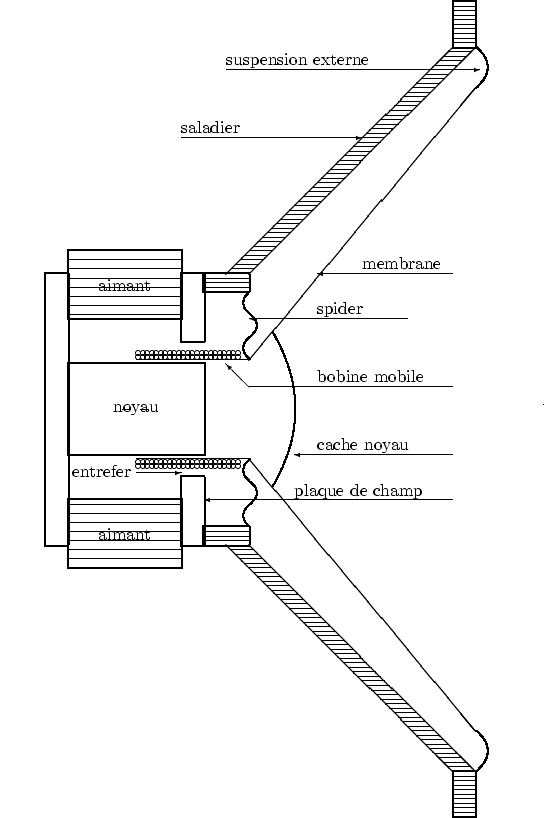
\includegraphics[width=0.3\textwidth]{figure/HP_schema_2}
	\hspace{2cm}
	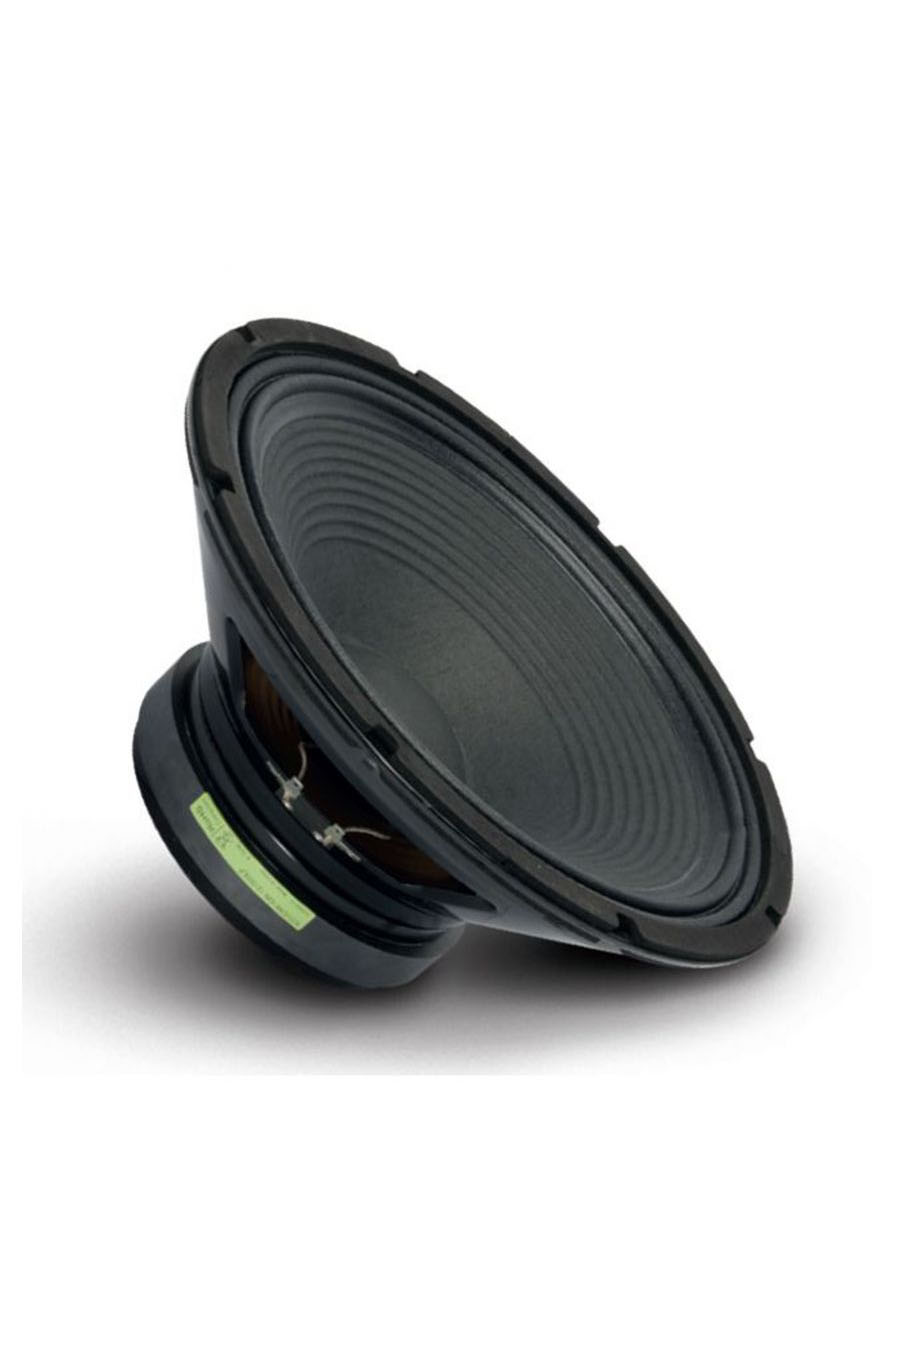
\includegraphics[width=0.3\textwidth]{figure/fane12-500lf.jpg}
	\end{center}
	\caption{Schéma d'un haut parleur, haut-parleur Fane 12-500LF}
	\label{HP_model}
\end{figure}
\end{frame}
\subsection{Electronique et Mécanique du haut parleur : Modèle linéaire classique}
\begin{frame}{Couplage électro-mécanique, force de Lorentz}
	La bobine, solidaire du haut-parleur, est plongée dans un champ magnétique dans l'entrefer du circuit magnétique. Celle-ci peut uniquement se déplacer dans l'axe de révolution du système physique. 
\begin{itemize}
	\item Un élément de fil de la bobine : $\mathrm dl$
	\item Le courant est suivant $\vec{e}_\theta$
	\item Vitesse des charges : $\vec{v} = -v \vec{e}_\theta$
	\item Champ magnétique constant est dirigé vers l'extérieur : $\vec{B} = B \vec{e}_r$.
	\item Champ électrique nul en tout point : $\vec{E} = 0$
\end{itemize}
\begin{columns}[t]\small
  \begin{column}{.5\textwidth}
  \begin{displaymath}
	\begin{array}{rcl}
	\vec{F}_L & = & \int_0^L q\vec{E} + q \vec{v}\wedge\vec{B} \, \mathrm dl \\
	& = & \int_0^L - q v\vec{e}_\theta \wedge B \vec{e}_r \, \mathrm dl \\
	& = & \underbrace{q\, v}_{=i} B \int_0^L  \vec{e}_x \, \mathrm dl \\
	& = & Bli \vec{e}_x
	\end{array}		
	\end{displaymath}
  \end{column}
  \begin{column}{.5\textwidth}
  \begin{figure}[!h]
	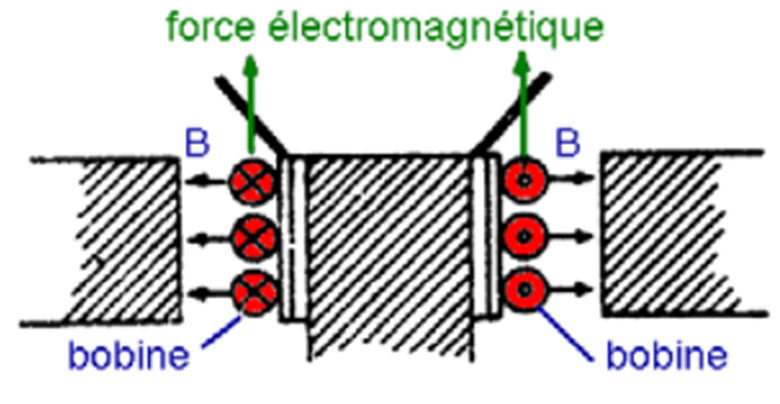
\includegraphics[width=0.5\textwidth]{figure/laplace_1.jpg}
	\caption{Schéma de la bobine d'un haut-parleur dans l'entrefer}
	\end{figure}
  \end{column}
\end{columns}


\end{frame}
\begin{frame}{Gyrateur : la bobine}
Le mouvement de la bobine dans le champ magnétique entraine une force tension $e$ ou force contre-électromotrice induite. 
Cette tension a pour expression $e = -Blv$.
Nous pouvons modéliser cette transformation par un gyrateur dont le rapport de transformation est à une quantité importante dans tout haut-parleur, le facteur $Bl$.
\begin{columns}[t]\small
  \begin{column}{.5\textwidth}
  	\vfill
	\begin{displaymath}
	\left( \begin{array}{c} F_L \\ \frac{dx}{dt} \end{array} \right)
	= \left( \begin{array}{cc} 0 & Bl\\ \frac{1}{Bl} & 0 \end{array} \right)
	\left( \begin{array}{c} e \\ i \end{array} \right)
	\end{displaymath}
  \end{column}
  \begin{column}{.5\textwidth}
	\begin{figure}[!h]
	\begin{center}
	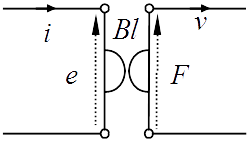
\includegraphics[width=0.4\textwidth]{figure/gyrateur.png}
	\end{center}
	\caption{Schéma de la bobine d'un haut-parleur dans l'entrefer}
	\label{gyrateur}
	\end{figure}	
  \end{column}
\end{columns}
\end{frame}
\begin{frame}{Circuit électrique}
Le circuit électrique d'un haut-parleur est très simple :
\begin{itemize}
	\item Résistance $R_{DC}$ du fil en série
	\item Inductance $L$ de la bobine en série
	\item Contre-réaction : $e=-Blv$
	\item Alimentation par un amplificateur supposé idéal : $v_{in}$
\end{itemize}
\begin{equation*}
	v_{in} = R_{DC}i + L \frac{di}{dt} + Blv
\end{equation*}
\begin{figure}[!h]
	\begin{center}
	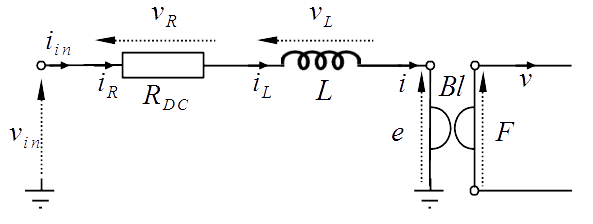
\includegraphics[width=0.6\textwidth]{figure/schema_elec.png}
	\end{center}
	\caption{Schéma de la partie électrique d'un haut parleur}
	\label{schema_elec}
\end{figure}
\end{frame}
\begin{frame}{Couplage mécano-acoustique}
Hypothèses : 
\begin{itemize}
	\item Membrane infiniment rigide.
	\item Haut-parleur assimilé à un piston plan de section $S$
	\item Force $F_p$ est la résultante des forces de pression appliquées à l'avant et à l'arrière de la membrane
	\item Différence de pression acoustique $p$
\end{itemize}
\begin{columns}[t]\small
  \begin{column}{.5\textwidth}
  	\vfill
	\begin{displaymath}
	\left( \begin{array}{c} p \\ u \end{array} \right)
	= \left( \begin{array}{cc} \frac{1}{S} & 0\\ 0 & S \end{array} \right)
	\left( \begin{array}{c} F_p \\ v \end{array} \right)
	\end{displaymath}
  \end{column}
  \begin{column}{.5\textwidth}
	\begin{figure}[!h]
	\begin{center}
	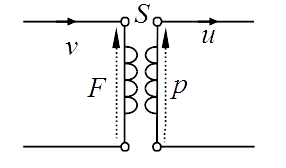
\includegraphics[width=0.6\textwidth]{figure/schema_meca2acoustique.png}
	\end{center}
	\caption{Schéma de la transduction du milieu mécanique vers acoustique}
	\label{schema_meca2acoustique}
	\end{figure}	
  \end{column}
\end{columns}

	

\end{frame}
\begin{frame}{Circuit mécanique}
\begin{itemize}
	\item Le spider et la suspension : raideur $k$, ou de compliance $C=\frac{1}{k}$ (non vérifié à forte amplitude). Force de rappel : $F_k = -k x$
	\item Forces de frottements fluides : $F_f = -R_f \frac{dx}{dt}$, la facteur $R_f$ n'est pas constant en fonction de la fréquence.
	\item Poids de la membrane négligé.
	\item Force de Laplace : $F_L = Bli$
	\item Forces de pression : $-F_p$
\end{itemize}
	Principe fondamental de la dynamique :
	\begin{equation*}
		m \frac{d^2 x}{dt^2} = F_f + F_k + F_L - F_p
	\end{equation*}
	\begin{equation*}
		m \frac{d^2 x}{dt^2} + R_f \frac{dx}{dt} + k x + F_p = Bli 
	\end{equation*}
	eeza
\end{frame}
\begin{frame}{Schéma électro-mécanique du haut-parleur}
	\begin{figure}[!h]
	\begin{center}
	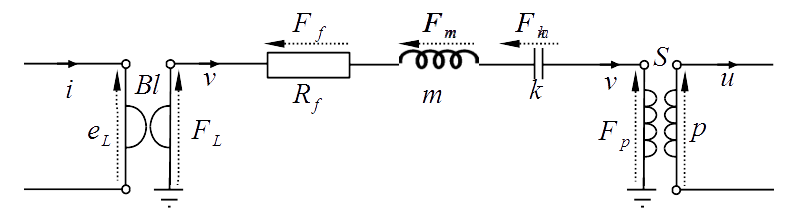
\includegraphics[width=1\textwidth]{figure/schema_meca.png}
	\end{center}
	\caption{Schéma de la partie mécanique d'un haut parleur}
	\label{schema_meca}
	\end{figure}	
\end{frame}
\begin{frame}{Impédance acoustique}
Hypothèses : 
\begin{itemize}
	\item Piston plan
	\item Champ libre à l'avant
	\item Charge close à l'arrière
\end{itemize}
\begin{columns}[t]\small
  \begin{column}{.6\textwidth}
  \begin{itemize}
  	\item Volume : $V$
  	\item Pression intérieure : $p$
  	\item Déplacement : $x$ (sens positif vers l'extérieur)
  	\item Au repos : $V=V_0$ et $p=0$
  	\item Section : $S$
  	\item Rayon $r$
  \end{itemize}
  \end{column}
  \begin{column}{.4\textwidth}
	\begin{figure}[!h]
	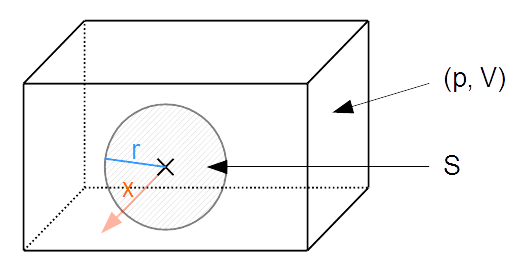
\includegraphics[width=1\textwidth]{figure/enceinte.png}
	\caption{Schéma d'une enceinte close}
	\end{figure}	
  \end{column}
\end{columns}
\end{frame}
\begin{frame}{Impédance de rayonnement de la face avant}
Impédance de rayonnement d'un disque infiniment rigide dans un plan infini (approximation)
\begin{equation}
	 Z_{ray}(j\omega) = j\omega m_a+\frac{1}{j\omega C_a}+r_a
\end{equation}
\begin{itemize}
	\item Masse acoustique $m_a$, 
	\item Raideur acoustique $C_a$
	\item Dissipation standard $r_a$
\end{itemize}
\end{frame}
\begin{frame}{Impédance de rayonnement de la face arrière}
Avec les approximations standardes de l'acoustique basse fréquence.
Hypothèse : 
\begin{itemize}
	\item Enceinte close
	\item Transformation adiabatique réversible : $P V^\gamma = cte$
\end{itemize}
\begin{columns}[t]\small
  \begin{column}{.5\textwidth}
  	\begin{displaymath}
		\frac{p}{P_0} + \gamma \frac{dV}{V_0} = 0
	\end{displaymath}
	\begin{displaymath}
		dV = Sx
	\end{displaymath}
  \end{column}
  \begin{column}{.4\textwidth}
 	\begin{displaymath}
		F_{p_{in}}= Sp
	\end{displaymath}
	\begin{displaymath}
		F_{p_{in}}= -\gamma\frac{P_0}{V_0}S^2 x
	\end{displaymath}

  \end{column}
\end{columns}
	En dérivant cette expression et en remplaçant force par pression et vitesse par débit, on obtient :
	\begin{equation}
		\frac{dp_{in}}{dt} = -k_{ac}u, \text{ avec $k_{ac}=\gamma\frac{P_0}{V_0}$}
	\end{equation}
	
	La partie acoustique se modélise donc par une capacité ($C_{ac}=\frac{1}{k_{ac}}$) en série avec une impédance, 
\end{frame}
\begin{frame}
	\begin{figure}[!h]
	\begin{center}
	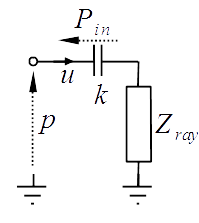
\includegraphics[width=0.3\textwidth]{figure/schema_acoustique.png}
	\end{center}
	\caption{Schéma d'une enceinte close}
	\label{schema_acou}
	\end{figure}	
\end{frame}
\begin{frame}{Paramètres de Thiele \& Small}	
	\begin{figure}[!h]
	\begin{center}
	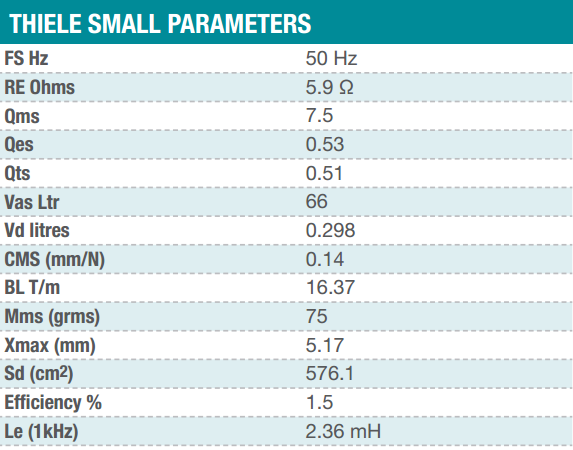
\includegraphics[width=0.59\textwidth]{figure/thieleSmallFane12500LF.png}
	\end{center}
	\caption{Paramètre de Thiele \& Small pour le Fane 12-500 LF}
	\label{ThieleSmall}
	\end{figure}	
	
\end{frame}
\begin{frame}{Représentation d'état classique}
	\begin{figure}[!h]
	\begin{center}
	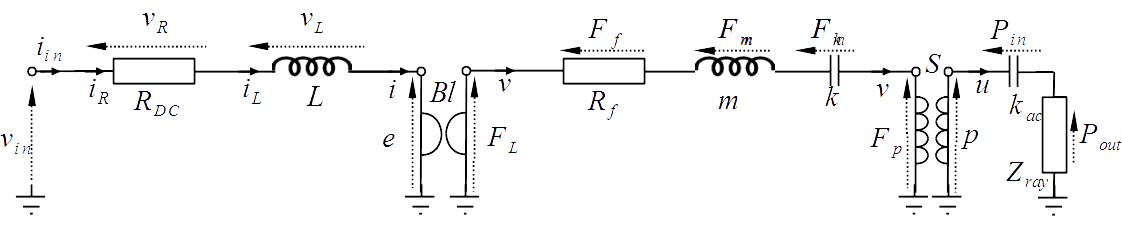
\includegraphics[width=1\textwidth]{figure/schema_general.png}
	\end{center}
	\caption{Schéma général du haut-parleur}
	\label{schema_gene}
	\end{figure}
\end{frame}




\section{Micro = (haut-parleur)$^{-1}$}
\subsection{Directivité des microphones}
\begin{frame}{Omnidirectionnel}
	\begin{figure}[!h]
	\begin{center}
	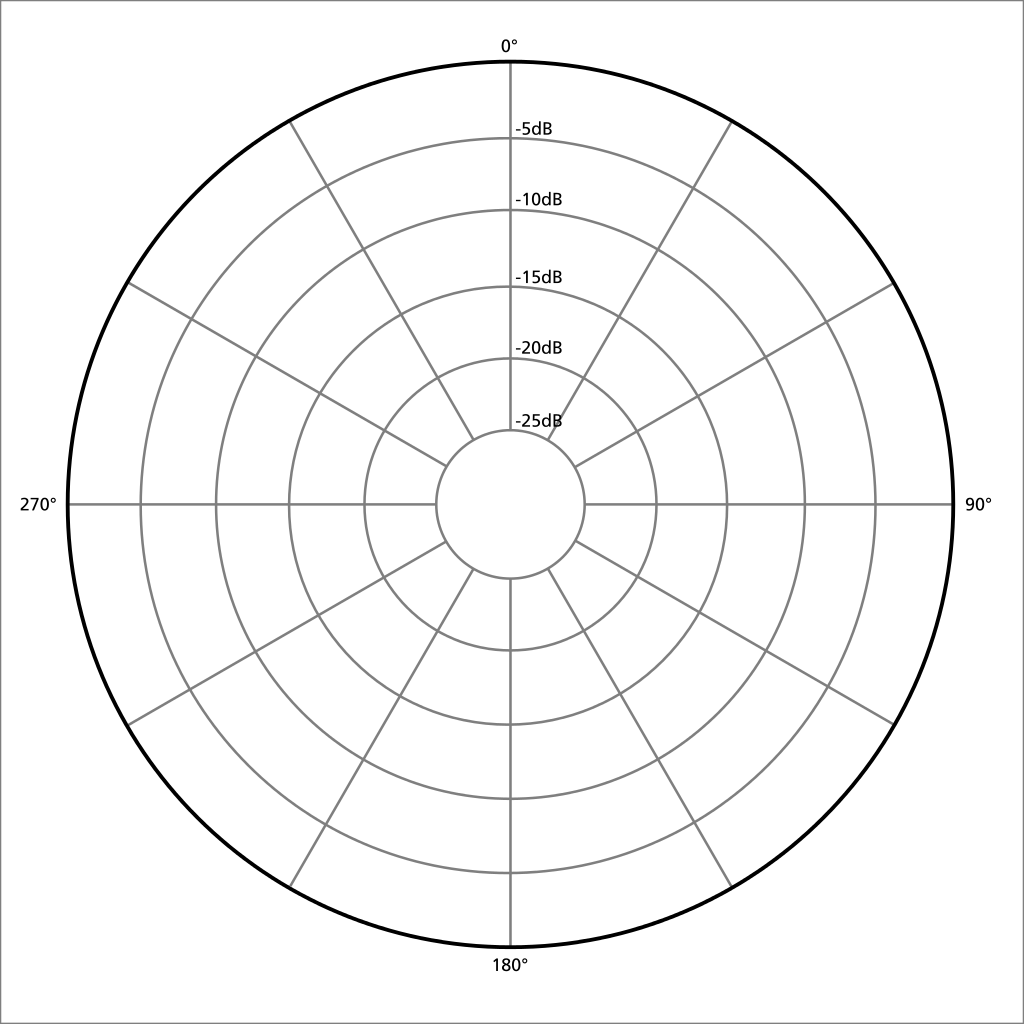
\includegraphics[width=0.4\textwidth]{figure/Polar_pattern_omni.png}
	\end{center}
	\caption{Diagramme Omnidirectionnel}
	\end{figure}
\end{frame}
\begin{frame}{Cordioïde}
	\begin{figure}[!h]
	\begin{center}
	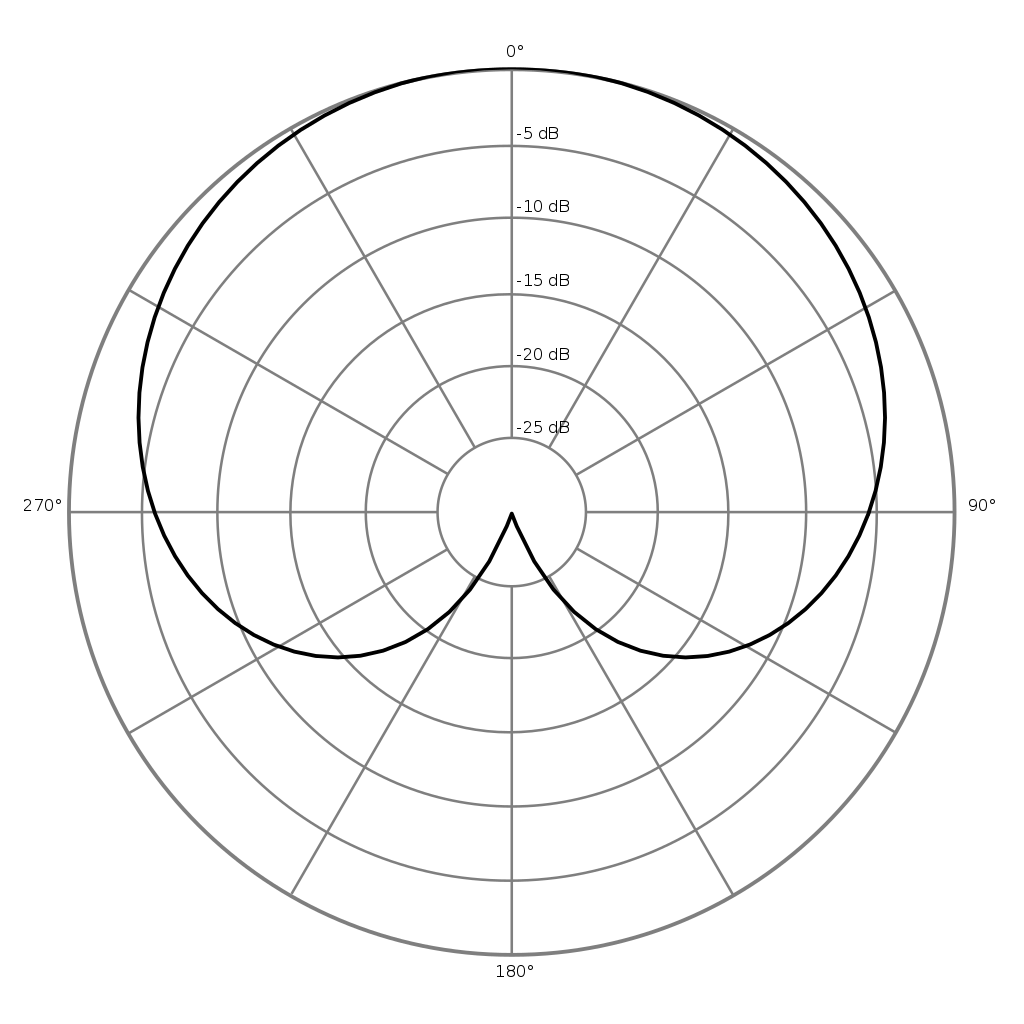
\includegraphics[width=0.4\textwidth]{figure/Polar_pattern_cardioid.png}
	\end{center}
	\caption{Diagramme Cordioïde}
	\end{figure}
\end{frame}
\begin{frame}{hypercardioïd}
	\begin{figure}[!h]
	\begin{center}
	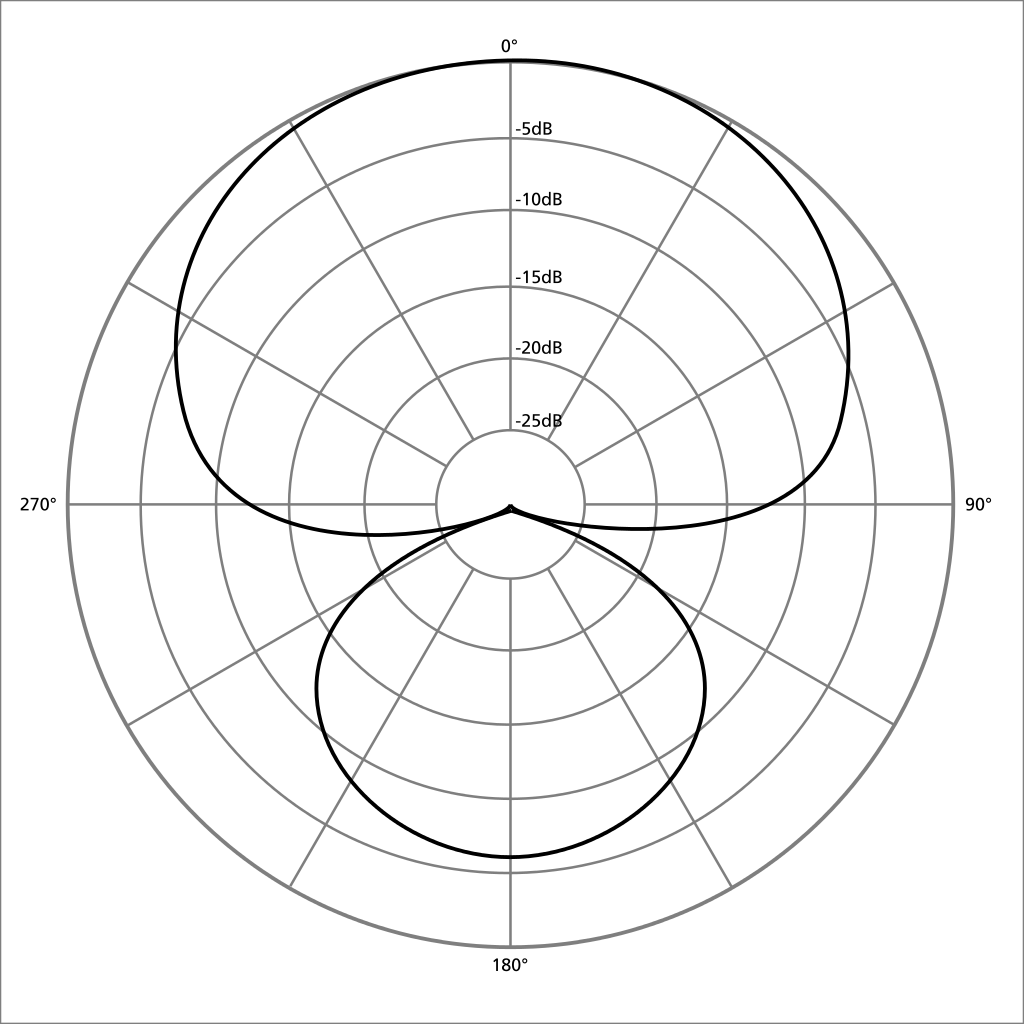
\includegraphics[width=0.4\textwidth]{figure/Polar_pattern_hypercardioid.png}
	\end{center}
	\caption{Diagramme }
	\end{figure}
\end{frame}
\begin{frame}{supercardioïde}
	\begin{figure}[!h]
	\begin{center}
	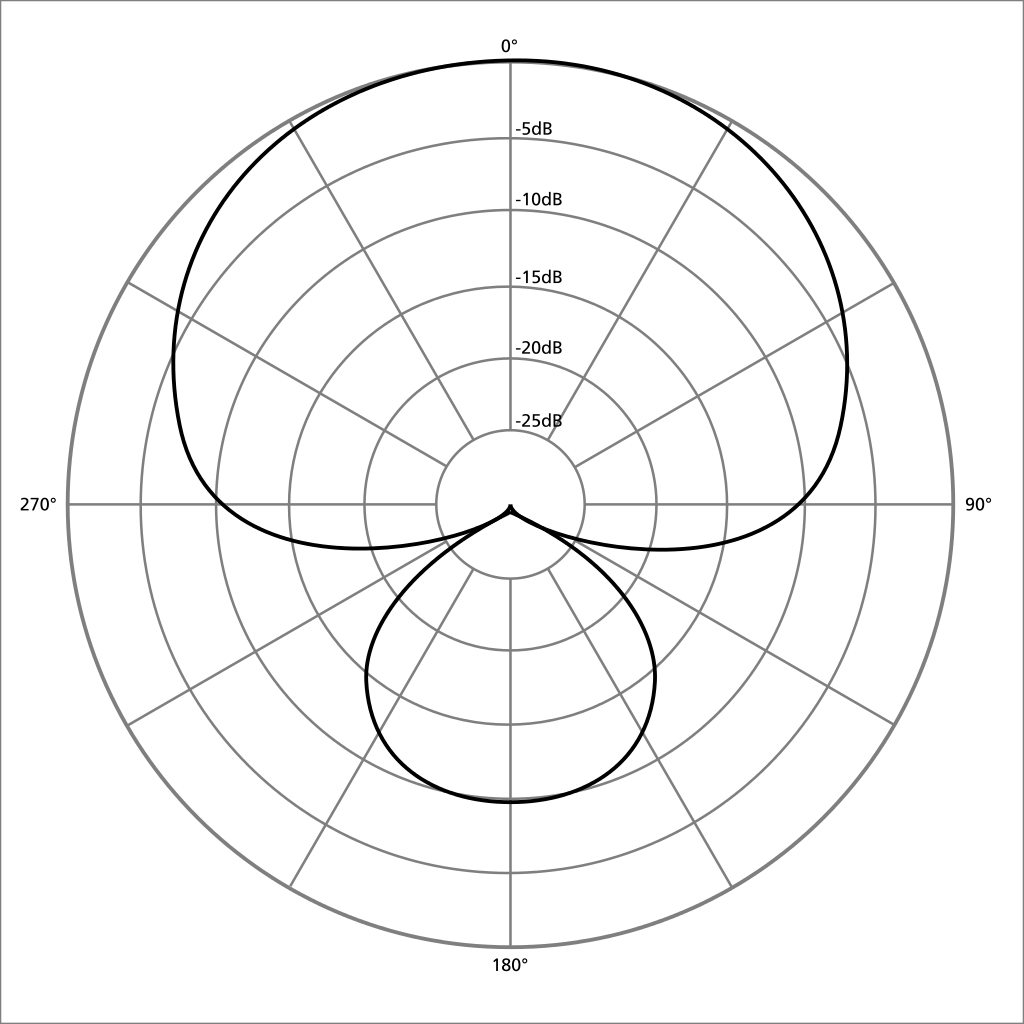
\includegraphics[width=0.4\textwidth]{figure/Polar_pattern_supercardioid.png}
	\end{center}
	\caption{Diagramme supercardioïde}
	\end{figure}
\end{frame}
\begin{frame}{Bidirectionnel}
	\begin{figure}[!h]
	\begin{center}
	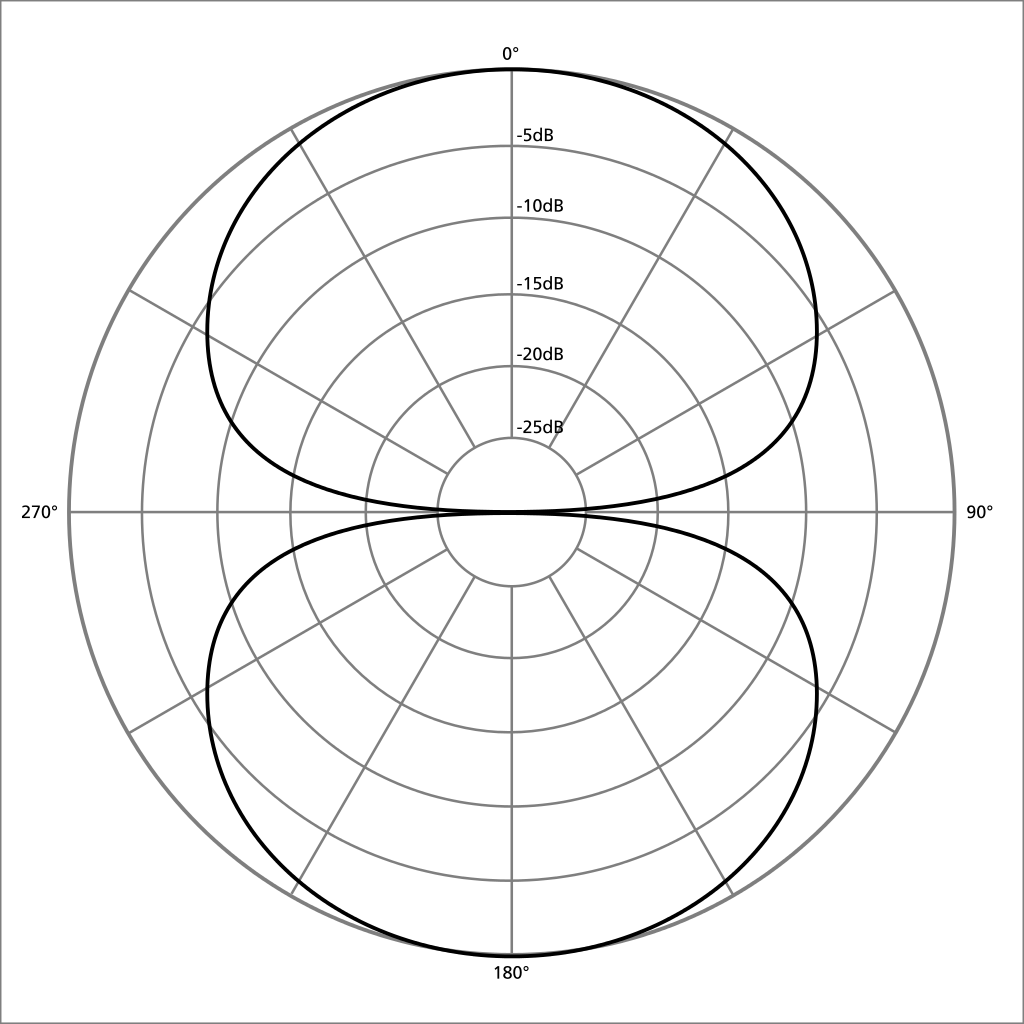
\includegraphics[width=0.4\textwidth]{figure/Polar_pattern_figure_eight.png}
	\end{center}
	\caption{Diagramme bidirectionnel}
	\end{figure}
\end{frame}
\begin{frame}{Test d'écoute}

	\begin{figure}[!h]
	\begin{center}
	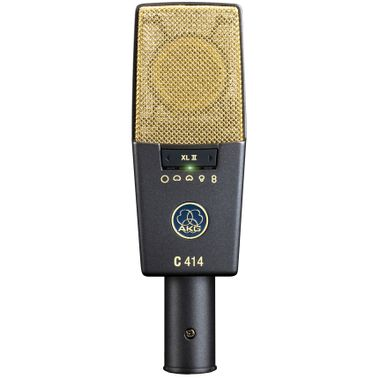
\includegraphics[width=0.4\textwidth]{figure/akg-c414-xlii-120450.jpg}
	\end{center}
	\caption{Micro AKG c414}
	\end{figure}
\end{frame}
\subsection{Dynamique, statique, à ruban}

\begin{frame}{Micro dynamique}
\begin{columns}[t]\small
  \begin{column}{.5\textwidth}
  Principe :
  \begin{itemize}
	\item Inverse d'un haut-parleur,
	\item Bobine collée à une membrane,  
	\item Flux magnétique généré par un aimant permanent,
  \end{itemize}
  \end{column}
  \begin{column}{.5\textwidth}
	\begin{figure}[!h]
	\begin{center}
	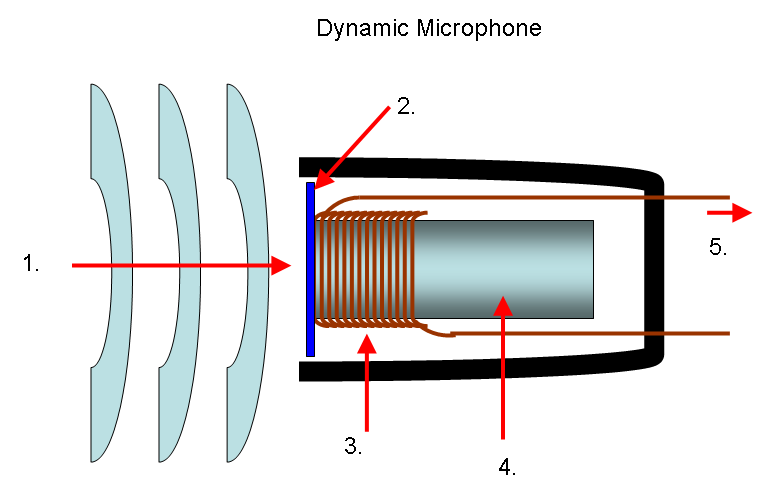
\includegraphics[width=.8\textwidth]{figure/Mic-dynamic.png}
	\end{center}
	\caption{Micro dynamique}
	\end{figure}
  \end{column}
\end{columns}
\end{frame}

\begin{frame}{Micro statique}
\begin{columns}[t]\small
  \begin{column}{.5\textwidth}
  Principe :
  \begin{itemize}
	\item Condensateur chargé dont l'une des armatures est mobile,
	\item Représenté par une capacité variable,
	\item Nécessite une alimentation dite fantôme,
	\item Nécessite un amplificateur proche de la membrane
	\item $C(e)=\epsilon\frac{S}{e}$ et $q(e) = C(e) V$
  \end{itemize}
  \end{column}
  \begin{column}{.5\textwidth}
	\begin{figure}[!h]
	\begin{center}
	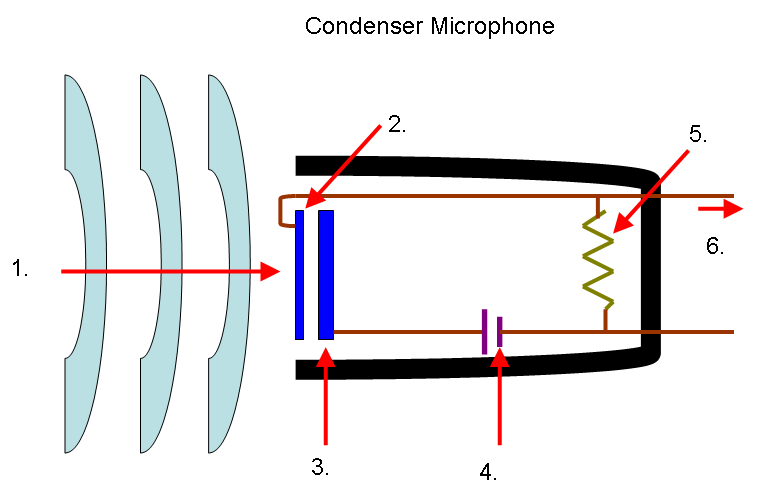
\includegraphics[width=.8\textwidth]{figure/Mic-condenser.png}
	\end{center}
	\caption{Micro statique}
	\end{figure}
  \end{column}
\end{columns}

La sensibilité des microphones électrostatiques est supérieure à celle des microphones dynamiques. 
\end{frame}

\begin{frame}{Micro à ruban}
\begin{columns}[t]\small
  \begin{column}{.5\textwidth}
Principe :
\begin{itemize}
	\item La membrane est un ruban gaufré souple, 
	\item Dans un champ magnétique d'un aimant permanent,
	\item Partie mobile très légère
	\item Impédance de sortie très faible 
	\item Extremement fragile.
\end{itemize}
  \end{column}
  \begin{column}{.5\textwidth}
	\begin{figure}[!h]
	\begin{center}
	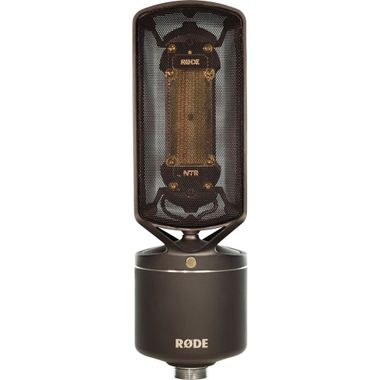
\includegraphics[width=.8\textwidth]{figure/ntr02.jpg}
	\end{center}
	\caption{Micro Rode NTR}
	\end{figure}
  \end{column}
\end{columns}

\end{frame}

\subsubsection{Plage de fréquences et réponse en fréquence}
\begin{frame}{Plage de fréquences et réponse en fréquence}
La plage de fréquences d’un micro détermine son aptitude à restituer les fréquences qu’il capte (par exemple les fréquences comprises entre 20 Hz et 20 kHz).
	\begin{figure}[!h]
	\begin{center}
	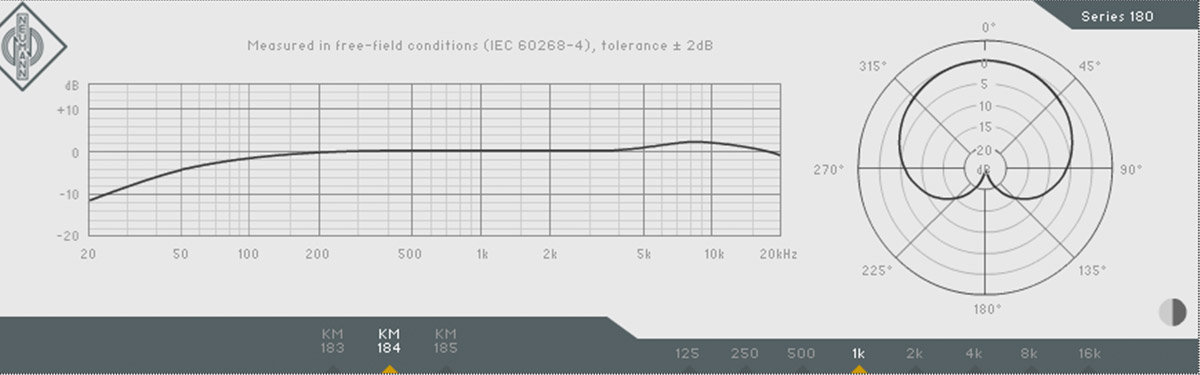
\includegraphics[width=1\textwidth]{figure/Diagramm-KM184.jpg}
	\end{center}
	\caption{Réponse en fréquence d'un micro KM184}
	\end{figure}
\end{frame}

\begin{frame}{Plage de fréquences et réponse en fréquence}
	\begin{figure}[!h]
	\begin{center}
	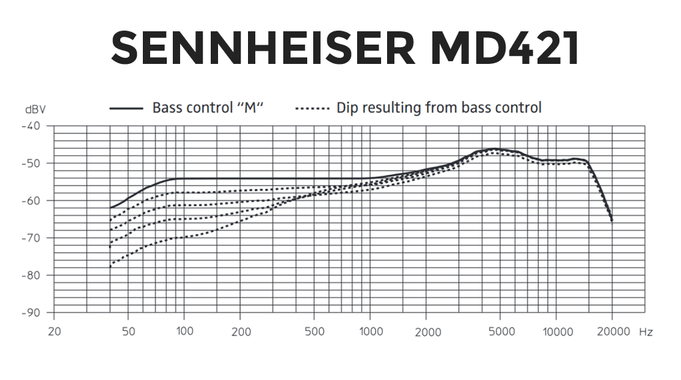
\includegraphics[width=0.8\textwidth]{figure/sennheiser-MD421.png}
	\end{center}
	\caption{Réponse en fréquence d'un micro MD421}
	\end{figure}
\end{frame}
\subsubsection{Sensibilité}

\begin{frame}{Sensibilité}
\begin{itemize}
	\item Tension de sortie fournie par le micro soumis à une pression acoustique
	\item Mesure prise à 1kHz
	\item $mV/Pa$ ou en $dBV/Pa$
	\item Ordre de grandeur : 
\begin{itemize}
	\item Shure Sm58 (dynamique) : $-56dBV/Pa$
	\item Neumann Km184 (statique) : $-36dBv/Pa$
\end{itemize}
\end{itemize}
\end{frame}

\subsubsection{Pression acoustique maximale}
\begin{frame}{Pression acoustique maximale}
\begin{itemize}
	\item La pression acoustique maximale indique le niveau maximum pouvant être supporté avant saturation de la membrane, voire de sa dégradation
	\item Mesure en dB SPL avec un taux de distorsion de $1\%$
	\item Ordre de grandeur : entre 110 et 150 dB.
\end{itemize}
\end{frame}

\subsubsection{Impédance de sortie}

\begin{frame}{Impédance de sortie}
\begin{itemize}
	\item Impédance de sortie du micro en $\omega$.
	\item Ordre de grandeur : 50 à 600 $\omega$
\end{itemize}
\end{frame}


\section{Système de sonorisation}
\subsection{Sonorisation d'un concert/festival}
\begin{frame}{HellFest ;)}
	\begin{figure}[!h]
	\begin{center}
	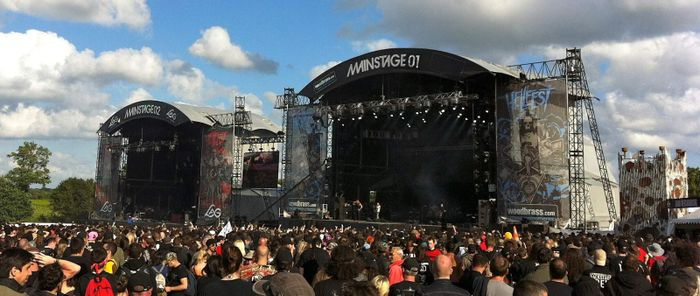
\includegraphics[width=1\textwidth]{figure/hellfest+main+stage.jpg}
	\end{center}
	\caption{HellFest 2013 : Mainstage}
	\end{figure}
\end{frame}

\subsection{En france, on est bon !}
\begin{frame}{En france, on est bon !}
\begin{columns}[t]\small
  \begin{column}{.33\textwidth}
  	\begin{figure}[!h]
	
\includegraphics[width=1\textwidth]{figure/nexo.jpg}
	\end{figure}
  \end{column}
  \begin{column}{.33\textwidth}
  	\begin{figure}[!h]
	
\includegraphics[width=1\textwidth]{figure/lacoustics.png}
	\end{figure}
  \end{column}
  \begin{column}{.33\textwidth}
	\vspace{1.5cm}
  	\begin{figure}[!h]
	
\includegraphics[width=1\textwidth]{figure/Logo-APG.jpg}
	\end{figure}
  \end{column}
\end{columns}
\end{frame}

\subsection{Caractéristiques d'un système de diffusion}
\begin{frame}{Qu'est-ce qu'une "bon" système son ?}
\begin{itemize}
	\pause
	\item Puissance acoustique uniformément répartie dans l'espace,
	\pause
	\item Cohérence dans l'espace de la réponse en fréquence,
	\pause	
	\item Réponse en fréquence plane,
	\pause	
	\item Absence de distorsion 
\end{itemize}
\end{frame}

\subsubsection{Puissance acoustique uniformément répartie dans l'espace}
\begin{frame}{Puissance acoustique uniformément répartie dans l'espace}
Problèmatique : la puissance sonore diminue avec la distance : 
  	\begin{figure}[!h]
	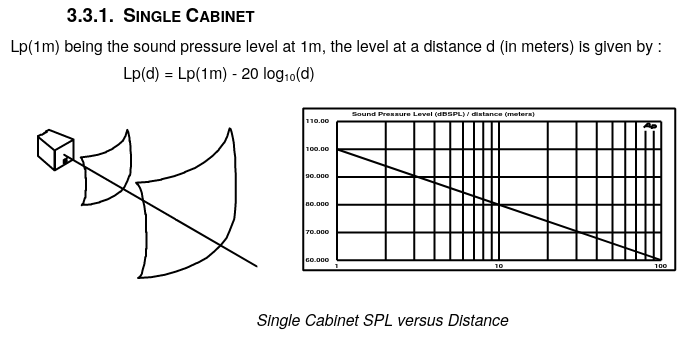
\includegraphics[width=0.8\textwidth]{figure/disp_sphere.png}
	\end{figure}
\end{frame}
\begin{frame}
  	\begin{figure}[!h]
	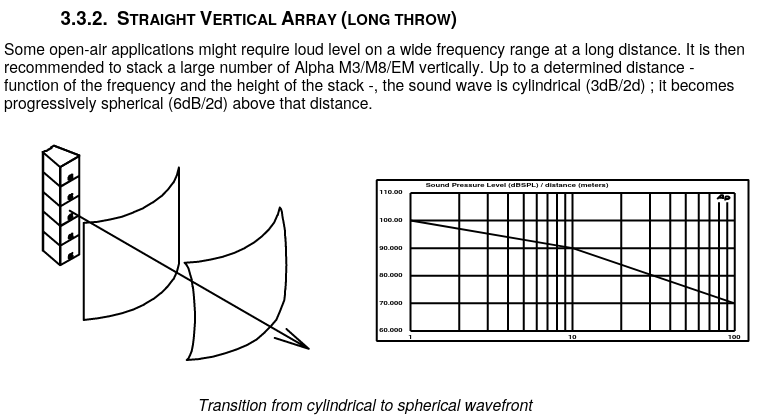
\includegraphics[width=0.8\textwidth]{figure/disp_cylindre.png}
	\end{figure}
\end{frame}
\begin{frame}
  	\begin{figure}[!h]
	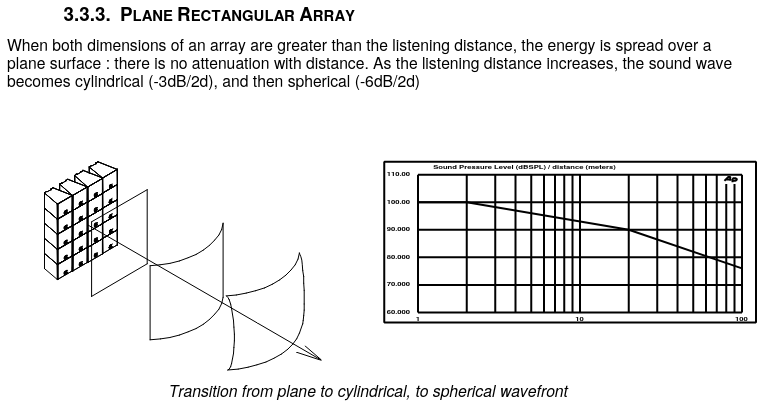
\includegraphics[width=0.8\textwidth]{figure/disp_plan.png}
	\end{figure}
\end{frame}

\begin{frame}{Le Linearray}
\begin{columns}[t]\small
  \begin{column}{.33\textwidth}
  	\begin{figure}[!h]
	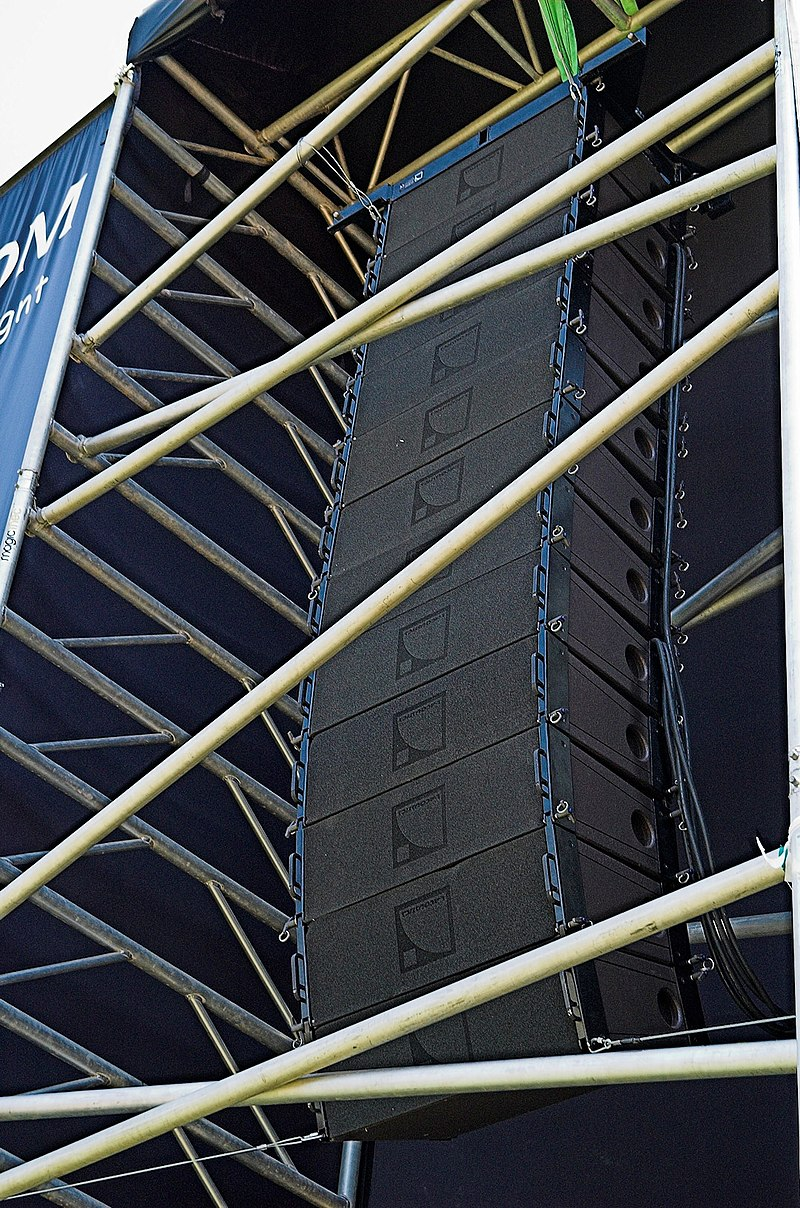
\includegraphics[width=0.8\textwidth]{figure/800px-L-Acoustics_DSC0908-02EC.jpg}
	\end{figure}

  \end{column}
  \begin{column}{.66\textwidth}
  	\vspace{2cm}
  	
	Réseau d'enceinte à une dimension pour la diffusion à longue portée.
  \end{column}
\end{columns}
\end{frame}

\begin{frame}
  	\begin{figure}[!h]
	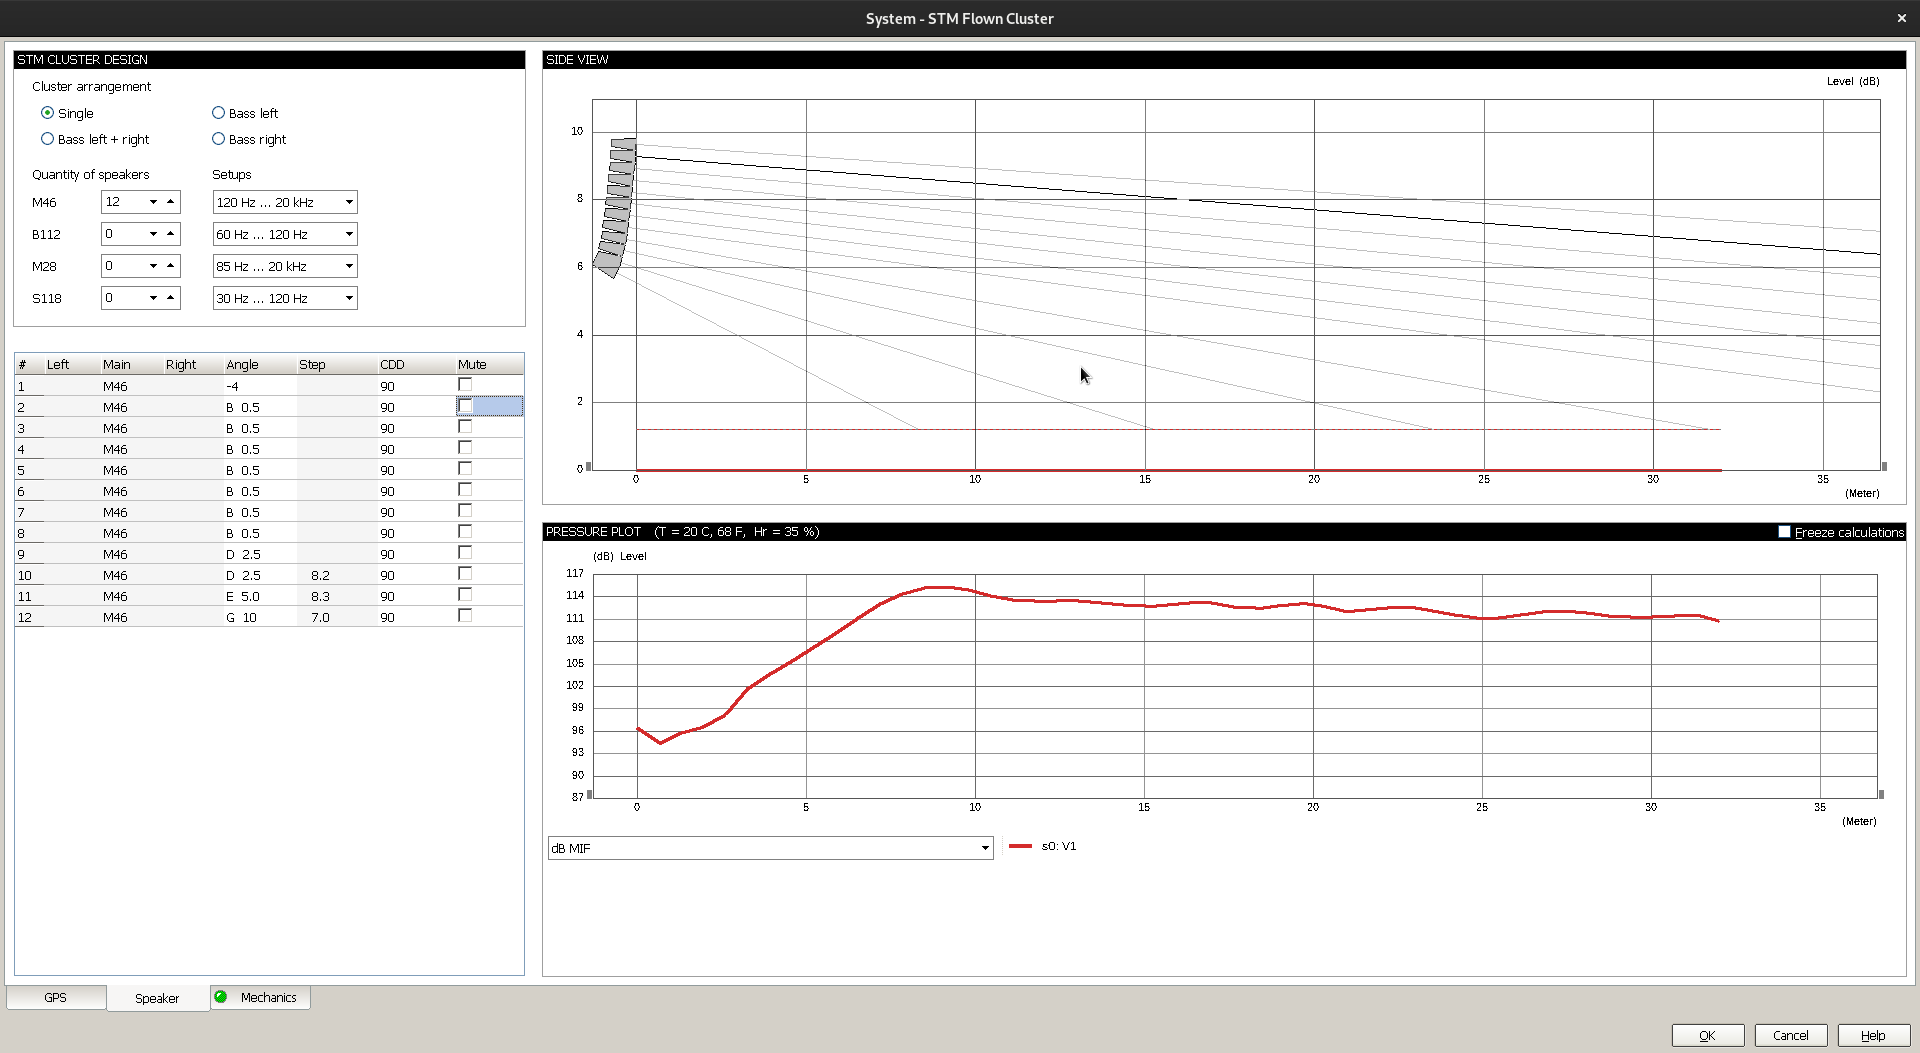
\includegraphics[width=1\textwidth]{figure/linearray_nexo.png}
	\end{figure}
\end{frame}

\subsubsection{Réponse en fréquence plane}
\begin{frame}{Réponse en fréquence plane}
\begin{itemize}
	\item Une fabrication correcte de base (choix des haut-parleurs, forme de l'enceinte, etc...)
	\item Enormément d'électronique pour le traitement du signal : Digital signal processig
\end{itemize}
\end{frame}

\subsubsection{Cohérence dans l'espace de la réponse en fréquence}
\begin{frame}{Cohérence dans l'espace de la réponse en fréquence}
\begin{itemize}
	\item Il faut que tout le spectre audio soit représenté pour l'ensemble des auditeurs
\end{itemize}
\end{frame}

\section{Simulation : système de subwoofer}
\subsection{Problématique}
\begin{frame}{Comment gérer les très basses fréquences ?}
Problème : 
\begin{itemize}
	\item Très très énergivore
	\item Omnidirectionnel (donc perte de puissance dans les zones où il n'y a pas de spectateurs)
	\item Limitation des rumble (larsen basse fréquence)
	\item Inconfort pour les musiciens
	\item Incohérence lors de la multiplication de sources
\end{itemize}
Solution : 
\begin{itemize}
	\item Système de spatialisation par interférences :
	\begin{itemize}
		\item Constructive pour l'audience,
		\item Destructive pour les musiciens,
	\end{itemize}
\end{itemize}
\end{frame}

\begin{frame}{Système classique}
	\href{https://www.nexo-sa.com/wp-content/uploads/NS1_v3305b18.zip}{Simulation}.
\end{frame}
\begin{frame}{Système endfire}
  	\begin{figure}[!h]
	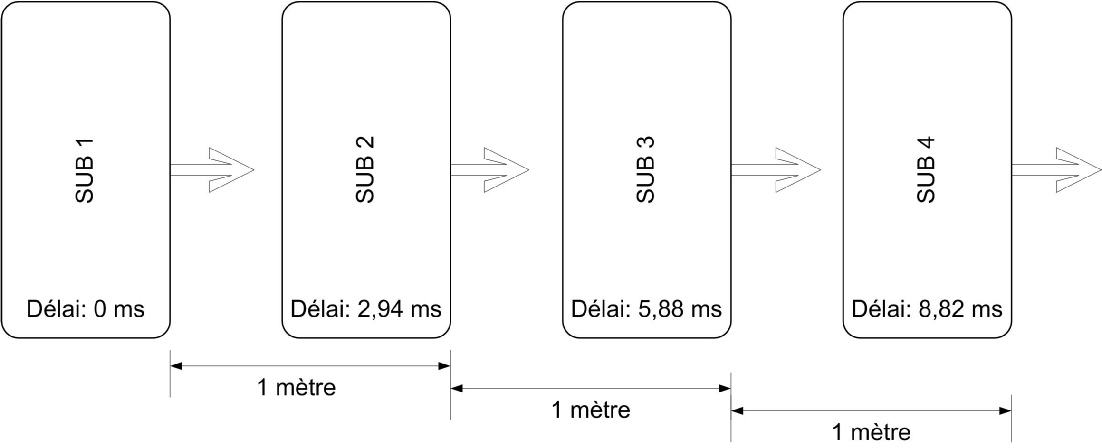
\includegraphics[width=1\textwidth]{figure/endfire3-1.jpg}
	\end{figure}
\end{frame}
\begin{frame}{Système endfire}
  	\begin{figure}[!h]
	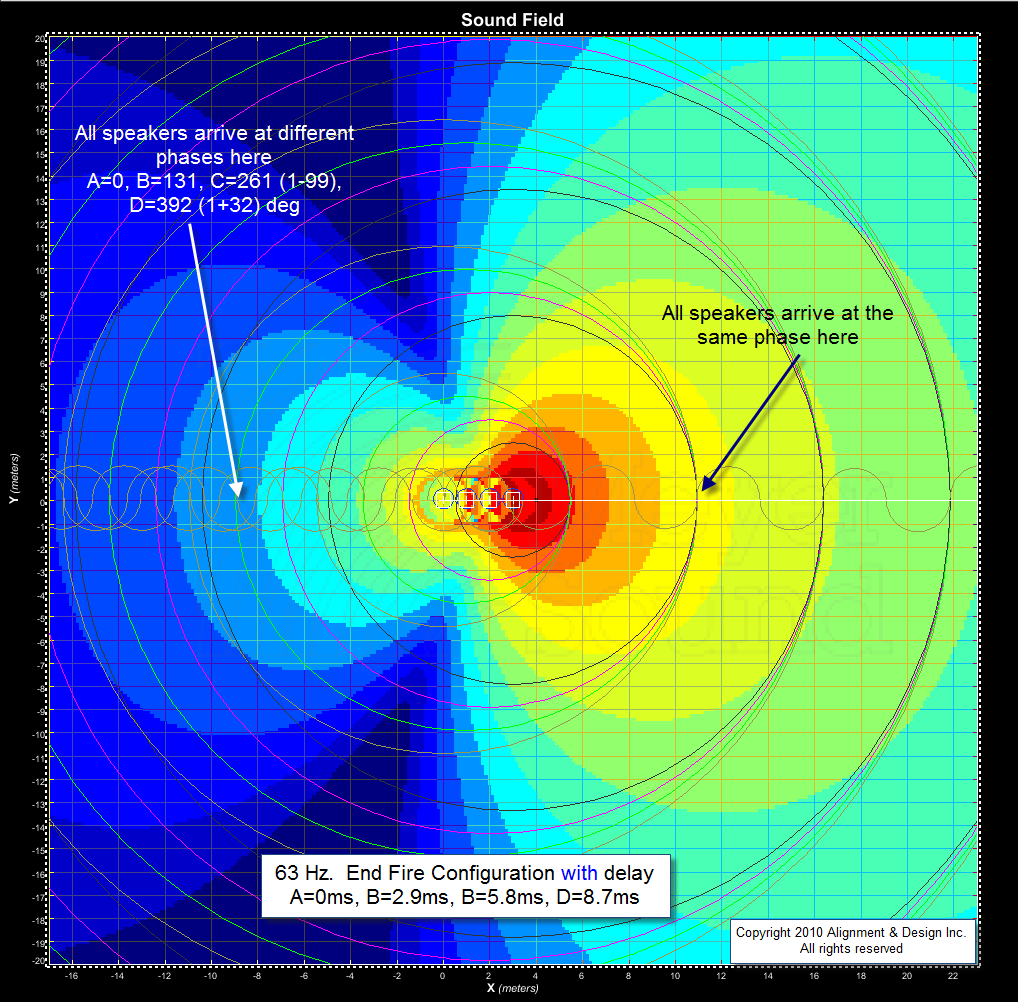
\includegraphics[width=0.5\textwidth]{figure/010b-end-fire-array-63-hz-1meter-with-2-9ms-delay-closeup.png}
	\end{figure}
\end{frame}


\end{document}
